\section{Encryption \& PKI}

% --- Slide 67: Contents ---
\begin{frame}{Contents}
    \Large
    \begin{enumerate}
        \color{gray}
        \item Introduction to Database Security Issues
        \item Discretionary Access Control (DAC)
        \item Mandatory Access Control (MAC)
        \item Role-Based Access Control (RBAC)
        
        \color{black} \bfseries
          \item Context-Based Access Control (CBAC)
    \end{enumerate}
\end{frame}

% --- Slide 68: Encryption (1) ---
\begin{frame}{Encryption (1)}
    \Large
    \begin{itemize}
        \setlength{\itemsep}{0.3cm}
        \item The \textbf{encoding of the data} by a special algorithm that renders the data \textbf{unreadable} by any program without the decryption key.
        
        \item \textbf{Symmetric cryptography}: sender and receiver use the \textbf{same key}.
        
        \item \textbf{Asymmetric cryptography}: encryption \& decryption keys are different (Public/Private keys).
    \end{itemize}
\end{frame}

% --- Slide 70: Encryption (3) - Sơ đồ Cryptosystem ---

\begin{frame}{Encryption (2)}
    \large
    \begin{itemize}
        \vspace{-0.05cm}
        \item \textbf{Symmetric (shared-/secret-key) cryptosystem}: the same key for (en/de)cryption algorithms ($K_E = K_D$).
        
        \vspace{0.05cm}
        \item \textbf{Asymmetric (public-key) cryptosystem}: public \& private keys ($K_E \neq K_D$).
    \end{itemize}
    
    \vspace{0.1cm}
    \centering
    % Bạn nhớ sửa tên file 'encryption3.jpg' thành đúng tên ảnh của bạn trong thư mục Assets nhé!
    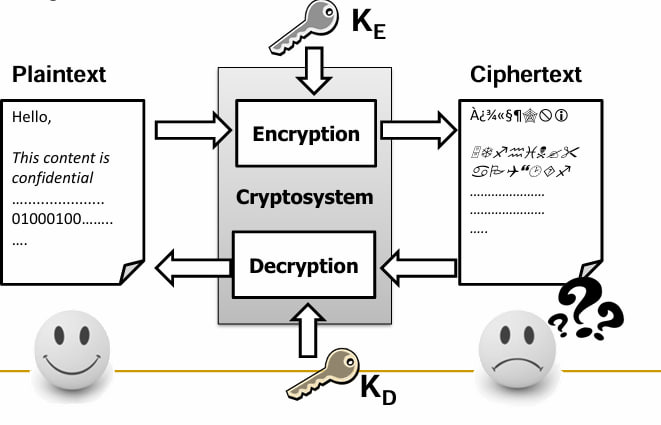
\includegraphics[width=0.6\textwidth]{Assets/encryption3.jpg}
\end{frame}






% --- Slide 74: Asymmetric techniques (1) ---
\begin{frame}{Asymmetric techniques (1)}
    \Large
    \begin{itemize}
        \item \textbf{RSA}: named after 3 inventors \textbf{R}ivest, \textbf{S}hamir, \textbf{A}dleman
        \begin{itemize}
            \large
            \item Two keys: \textbf{public key} and \textbf{private key}
            \item Public key is used for encryption.
            \item Private key is used for decryption.
        \end{itemize}
    \end{itemize}

    % Khoảng trống dương đẩy hình xuống dưới chữ (tuyệt đối không dùng dấu âm)
    \vspace{0.05cm} 
    
    \centering
    % Tôi để 0.85 để hình to vừa đủ, nếu thấy to quá bạn hạ xuống 0.75 nhé
    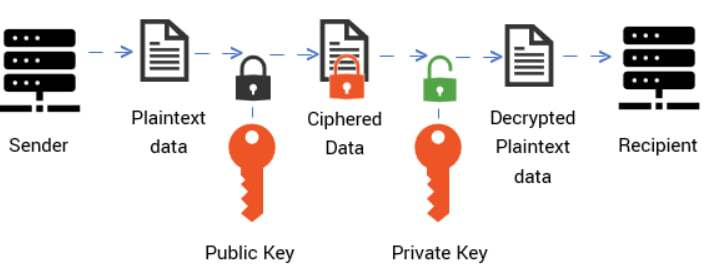
\includegraphics[width=0.85\textwidth]{Assets/encryption4.png}
\end{frame}


% --- Slide 75: Asymmetric techniques (2) ---
\begin{frame}{Asymmetric techniques (2)}
    \Large
    \begin{itemize}
        \item Encryption key: \textbf{public key}
        \item Decryption key: \textbf{private key}
        
        \vspace{0.3cm}
        \item Asymmetric techniques: \textbf{more secure} but \textbf{expensive} in terms of computational costs.
    \end{itemize}
    
    \vspace{0.5cm}
    \centering
    % Sơ đồ minh họa quy trình (Vẽ lại bằng TikZ)
    \begin{tikzpicture}[
        node distance=0.5cm,
        process/.style={rectangle, draw=green!60!black, thick, fill=white, text width=6cm, align=center, rounded corners, font=\small},
        arrow/.style={->, >=stealth, ultra thick, color=orange!80!black}
    ]
        % Node Sender
        \node[font=\bfseries\large] (sender) {Sender};
        
        % Node Quy trình ở giữa (Mô phỏng 2 hộp text như slide gốc)
        \node[process, right=1cm of sender] (box) {
            Use \textbf{public key} of receiver \\ to encrypt the message encryption key
            \par\vspace{0.2cm}\hrule\vspace{0.2cm}\par
            Encrypted message \\ using a \textbf{symmetric key}
        };
        
        % Node Receiver
        \node[font=\bfseries\large, right=1cm of box] (receiver) {Receiver};
        
        % Mũi tên kết nối
        \draw[arrow] (sender) -- (box);
        \draw[arrow] (box) -- (receiver);
        
    \end{tikzpicture}
\end{frame}


% --- Slide 76: Public Key Infrastructure (PKI) (1) ---
\begin{frame}{Public Key Infrastructure (PKI) (1)}
    \centering
    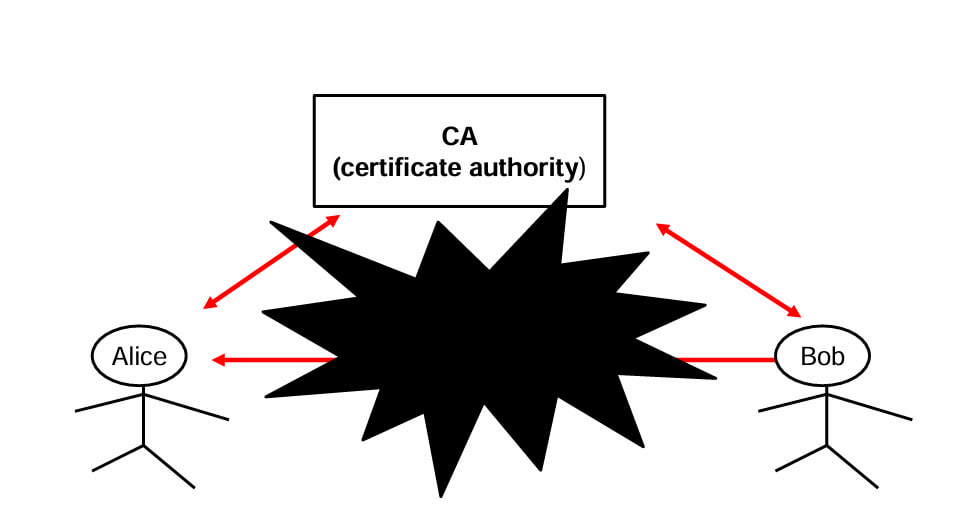
\includegraphics[width=0.9\textwidth]{Assets/publickey.jpg}
\end{frame}

% --- Slide 77: Public Key Infrastructure (PKI) (2) ---
\begin{frame}{Public Key Infrastructure (PKI) (2)}
    \Large
    \textbf{How does PKI work?}
    \vspace{0.2cm}
    
    \centering
    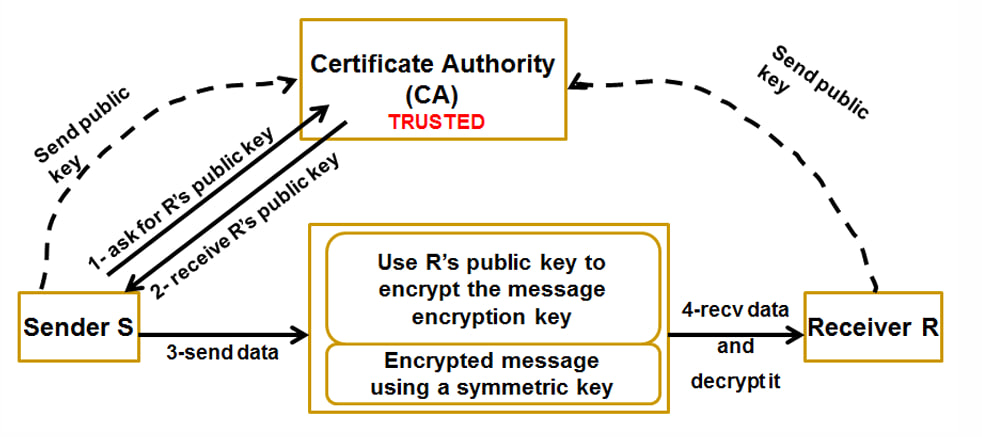
\includegraphics[width=0.9\textwidth]{Assets/publickey2.jpg}
    
\end{frame}


% --- Slide 78: Digital Signatures ---
\begin{frame}{Digital Signatures}
    \Large
    \begin{itemize}
        \item A \textbf{digital signature} is an example of using encryption techniques to provide authentication services in e-commerce applications.
        
        \vspace{0.2cm}
        \item A digital signature is a means of associating a mark \textbf{unique to an individual} with a body of text.
        \begin{itemize}
            \large
            \item The mark should be \textbf{unforgettable}, meaning that others should be able to check that the signature does come from the originator.
        \end{itemize}
        
        \vspace{0.2cm}
        \item A digital signature consists of a string of symbols.
        \begin{itemize}
            \large
            \item Signature must be \textbf{different for each use}.
            \item This can be achieved by making each digital signature a function of the message that it is signing, together with a \textbf{time stamp}.
        \end{itemize}
        
        \item Public key techniques are the means creating digital signatures.
    \end{itemize}
\end{frame}

% --- Slide 79: How digital signature works? (Placeholder Image) ---
\begin{frame}{How digital signature works?}
    \Large
    \textbf{Process flow:}
    
    \vspace{-0.2cm}
    \centering
    % KHUNG CHỪA TRỐNG ĐỂ BẠN CHÈN HÌNH SAU
    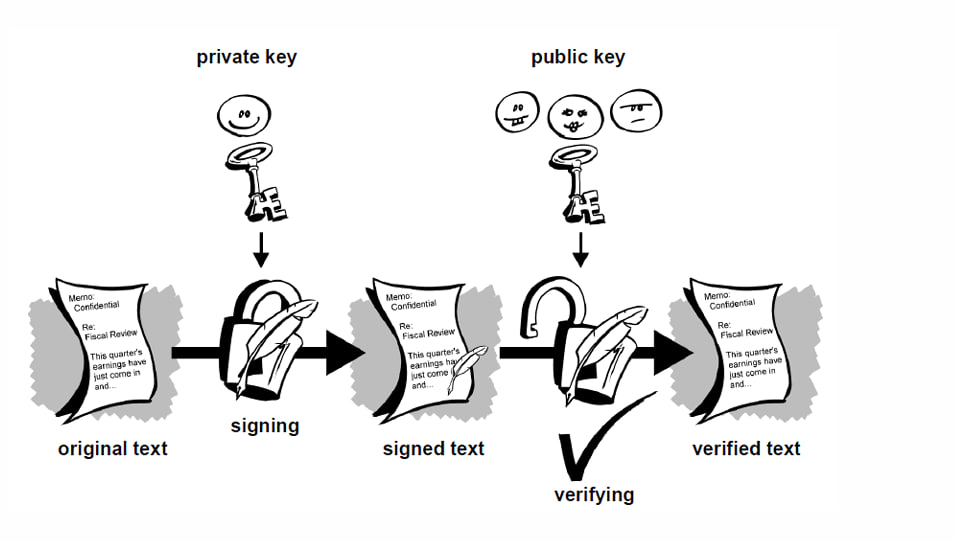
\includegraphics[width = 0.85\textwidth]{Assets/flow.jpg}
\end{frame}

% --- Slide 80: Digital certificates ---
\begin{frame}{Digital certificates}
    \Large
    \begin{itemize}
        \item \textbf{One concern} with the public key approach: must ensure that you are encrypting to the \textbf{correct person's public key}.
        
        \vspace{0.3cm}
        \item A solution: \textbf{digital certificates}.
        
        \vspace{0.3cm}
        \item A form of \textbf{credentials} (like a physical passport).
        
        \item Included with a person's public key to \textbf{verify that a key is valid}.
    \end{itemize}
\end{frame}

% --- Slide 81: Components of a digital certificate ---
\begin{frame}{Components of a digital certificate}
    \Large
    \begin{itemize}
        \item A digital certificate contains:
        \begin{itemize}
            \large
            \setlength{\itemsep}{0.2cm}
            \item A \textbf{public key}.
            \item \textbf{Certificate info} (identifying information such as name, ID).
            \item One (or more) \textbf{digital signatures}.
        \end{itemize}
        
        \vspace{0.5cm}
        \item Certificates are used when it is necessary to \textbf{exchange public keys} with someone (when you cannot manually exchange via a diskette or USB drive).
    \end{itemize}
\end{frame}

% --- Slide 82: Summary ---
\begin{frame}{Summary}
    \Large
    \begin{enumerate}
        \setlength{\itemsep}{0.4cm}
        \item Introduction to Database Security Issues
        \item Discretionary Access Control (DAC)
        \item Mandatory Access Control (MAC)
        \item Role-Based Access Control (RBAC)
        \item Encryption \& PKI (Public Key Infrastructure)
    \end{enumerate}
\end{frame}